\documentclass{article}
\usepackage{graphicx}
%\usepackage{fullpage}
\usepackage[margin=1.7in]{geometry}
\usepackage{wrapfig}
\newcommand{\degree}{\ensuremath{^\circ}}
\title{Artist Classification with Stylometry and Support Vector Machines}
\author{Ari Brown, Drew Gleeman, and Mike Micatka}
\date{\today}
\begin{document}
  \maketitle

  \section{Introduction}
  \subsection{Problem}
  The problem with being STEM students is that we have an incredibly poor ability
  to recognize artists from paintings. However, as with most problems in the
  modern age, they are easily solved with computers and math. Our specific problem
  is: given a painting and two possible artists, which artist made the painting?
  The problem itself is interesting although not important. It approaches the
  field of forgery detection, as our project is forgery detection at its most
  basic level: artist classification. We are going about this project by using a machine learning algorithm (Support
  Vector Machine, SVM) to make an educated estimate on who the artist is. With
  zero training, the computer would make simply a random guess. To turn this guess
  into an educated estimate, we train it on data from seven different features of
  each painting, telling the computer to which artist the features belong to.
  SVM can only make a decision based on one feature, so we run the SVM once for
  each feature and then we combine the outcomes of each feature using a weighted
  voting algorithm, where each feature's result gets a certain number of votes,
  and the winner is then declared by the program with a ``sureness'' factor.

  \subsection{Previous Work}
  There was a similar project done by undergraduate students at Stanford
  University in a machine learning class that focused on the machine learning
  aspect. Blessing and Wen used twelve different features to classify their
  data, with overlap on five of them with ours. Coincidentally, they chose to
  use the same machine learning algorithms as we did, which were a Bayesian
  Analyzer and Support Vector Machines. Our implementation differs from the reference implementation because we use
  fewer features to base our artist-selection decisions on, and we have
  different weights for our final decider. Trivially, we also used different
  data, overlapping with only two of the artists. Our implementation is better than the reference implementation because we
  make use of a weighted council-like approach to produce a single answer
  based on all of our stylometrics. We also use cross validation to get better
  training and more generalized results.

  \section{Technical Solution}
  \subsection{Summary}
  Our program is simple to use. Some time before testing and training are to be
  done, we run the produce\_features script. This computationally intensive
  script generates data for all features for all images and saves it in the
  features folder. Once completed, we run our program. It accepts two artists as
  input as well as a vector representing the weights of each feature, and
  returns the correct classification rates for each artist, using
  cross-validation.

  \subsection{Data}
  We chose four artists (Rembrandt, Pollock, Monet, and Picasso) and selected
  roughly 100 works from each artist. We chose each artist for their fame and
  peculiarities. Picasso was an interesting artist to choose, simply because his
  style has ranged from realism as a youth to cubism later in his life.
  Rembrandt is an artist we had seen mentioned in many papers, so we figured
  that it would be important to include him in our work. Pollock was chosen as
  he was an abstract painter with creative uses of colors that focused around a
  certain theme. Monet was selected as he was an impressionist painter who did
  many plein-air landscapes.

  \subsection{Weighted Combination}
  On a more technical level, the program also takes information on the weights
  of each feature and the threshold for ``sureness'', in which if the resulting
  sureness fails to meet the sureness, the program will produce a symbol which
  equates to not knowing. As each individiual stylometric feature gives its
  opinion on which artist produced the painting, the program weights the result
  as 0 or 1, depending on the determined artist. When all the stylometries have
  produced a result, the values are then weighted respectively according to the
  inputted weight matrix. The weighted values are then summed, and the final
  output is compared with the ``sureness'' threshold, and a final decision on
  the artist is produced. This process is completed for each painting. To speed
  this process, the stylometric data, an invariant, is produced ahead of time
  and stored in a handwritten file-system database. \\

  \subsection{Cross Validation}
  In the initial implementation of our algorithm, we arbitrarily split our
  images into two equal-sized groups - one for training and one for testing. The
  algorithm was then trained on the training data, with its performance being
  measured on the testing data. However, this naive implementation introduces
  some weaknesses. Only half of the data is used for training, so the results of
  the testing data are biased to reflect this. One common workaround for this
  problem is known as cross-validation. In \emph{k-fold} cross-validation, the
  data is divided into \emph{k} subgroups. Then, each subgroup is used as the
  testing data exactly once, with all of the rest of the subgroups being used as
  the training data. The results from the k iterations of the algorithm are then
  combined (in our case, averaged) in order to generate a more robust statistic
  for measuring the performance of the algorithm.

  \subsection{Histogram of Oriented Gradients}
  The histogram of oriented gradients stylometric, or HoG, is based on the
  direction of intensity changes in cells across an image. The idea behind it is
  that changes in intensity mark feature changes, and so a histogram for a small
  cell is produced based on each pixel. The histograms of each cell are then
  compiled into one, which is the final stylometric result. Which used a
  handwritten implementation that was heavily influenced from a different
  source.

  \subsection{Edge Detection}
  Our edge histogram algorithm was an adaptation of the Harris corner detection
  algorithm that was written for one of the homeworks. The Harris algorithm
  looks at two eigenvalues for every point, in order to determine if the point
  is part of a corner, edge, or flat surface. In our version of the algorithm
  for this, we care only about the larger of the two. For each point, we
  calculate the eigenvalues and select the largest one. We add that to a list,
  with one eigenvalue for each point. We then normalize the list by dividing by
  the largest value in it. All of the new values are then between 0 and 1. The
  final result of the algorithm is a histogram with four bins, representing the
  breakdown of the "corner sharpness" for all points in the image. The theory is
  that an artist who uses well-defined lines will have more points with large
  eigenvalues, where as an artist with blurry lines will have more low-value
  points. 

  \subsection{Local Binary Patterns}
  Local Binary Patterns are patterns that appear in numbers when checking the
  intensity of individual pixels. It is commonly used in texture identification,
  so the logic behind using it is that it would identify pixelated artwork such
  as that which Seurat is famous for (although Seurat's paintings were not used
  in this project). We used a handwritten implementation.

  \subsection{Corner Detection}
  Corner detection simply detects corner in the image. We used a handwritten
  implementation the detects the corners for a given threshold. The logic behind
  using this stylometric is that we will be able to tell if an artist prefers to
  use sharp contrast in two directions in their work. It is an extension of Edge
  Detection, in that regard. \\

  \subsection{Color Histogram}
  We did not expect much from this stylometric, but wanted to include it because
  it could shed light on an artist's overall color intensity. It was calculated
  by averaging the red, green, and blue values, respectively, for all pixels.
  The overall intensity of each pixel was also calculated. The motivation behind
  this was to observe an artist's overall intensity, as aforementioned, but also
  to discern any color preferences, however slight. \\

  \subsection{SIFT}
  SIFT or scale-invarient feature transform is an algorithm that is used to
  describe and locate features in images. The first part of this algorithm
  involves finding the keypoints which is done by finding the extrema of
  the Difference of Gaussians (DoG) at different scales. \\

  The SIFT algorithm used here is from the VLFeat library. When run, it finds
  different features and represents them as a 128-dimensional vector. We combined all of the SIFT features from our training set and clustered them into 10 different groups using k-means
  clustering. We then generated histograms of frequency for all of the images,
  both
  training and testing alike, of each of the feature clusters found in the
  training
  images of both artists. We can then use the histograms of the training set to
  train the SVM and the histograms of the testing images to classify using the
  trained SVM. \\

  In the VLFeat library, the default SIFT() call performs SIFT feature detection
  for a variety of scale spaces. In the SIFT algorithm, the scale space
  describes the size of the Gaussian kernel used to smooth the image. Larger
  scale sizes yield a more smoothed image. In our analysis, we perform SIFT
  feature detection at a variety of levels in order to more fully analyze the
  image. We perform the above analysis with a variety of different scale spaces
  in order to better differentiate between artists. This is useful for art
  identification because
  the different styles of artists can be subjectively determined by the patterns
  that exists at multiple levels, from brushstrokes to the overall theme of a
  painting. Our algorithm performs SIFT detection with scale spaces ranging from
  3 (the default) to 8 (the best-performing version of the algorithm, in our
  findings). To avoid displaying too much data, we show only the results from
  scale spaces 3 and 8, in our graphs. 

  \subsection{Blob Detection}
  Blob detection is a technique in which we calculate the centers of points of
  interest that have large intensity changes. The radius of a blob measures
  how far that intensity goes before changing drastically. This means it would
  be a great stylometric for measuring the presence of overall features that
  would mark a painting as visually distracting, such as still lives and Van
  Gogh's famous sunflower painting. \\

  \subsection{Fourier Spectral Analysis}
  Fourier Spectral Analysis is a common technique that was suggested to us by
  Dr. Dan Rockmore as a replacement for blob detection. Fourier spectral
  analysis returns Fourier coefficients for the image, where low frequency
  values represent background and high frequency values represent foreground
  and texture. The resulting matrix is in the shape of the original image
  (with the pixels having a change of basis performed on them, so the values
  do not match up at all), which means it is impossible to train the SVM
  algorithm on the raw FSA data. As an attempt to solve this, we tried taking
  the covariance of the data, which also unfortunately returned a matrix that
  was ultimately based on the size of the original image. We decided not to include Fourier spectral analysis in our final form
  because we could not figure out a way to faithfully represent the Fourier
  coefficients, and the overall results were not good enough to be included;
  they were little more than random guesses.

  \section{Experiments}
  In Figure 1, one can see the comparison of each feature's
  success in identifying the artist that a painting belonged to. SIFT 8, SIFT
  3, and blob detection were the three best individual features, and the overall
  weighted total also performs just as well as the SIFT 8 does. We ran multiple
  SIFT versions, but we chose to only display 3 and 8 because 3 was the minimum
  and 8 was the best. Judging from the fact that corner threshold checking was
  little better than random guessing, we can determine that these two artists
  used the same amount of corners and sharp color contrasts. LBP successfully
  identified many Monet paintings, which would suggest that there are textural
  differences between the way Monet routinely painted and the way Picasso
  painted. Picasso may have overlapped Monet's style, but it was not a routine
  fact.
  \begin{figure}[h!]
    \begin{center}
      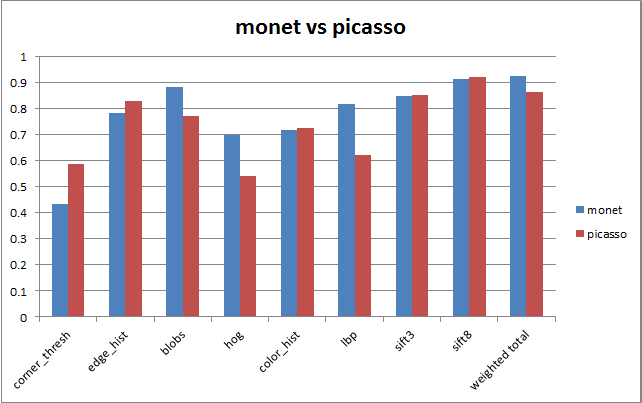
\includegraphics[width=3.5in]{graphs/monet_picasso.png}
      \caption{Monet vs Picasso}
    \end{center}
  \end{figure} \\

  Figure 2 shows just how different the two
  artists are, with almost every stylometry measuring distinct differences and
  styles. Yet again, SIFT outperformed the rest of the stylometries, and the
  overall weighting was hardly better than SIFT alone, but the interesting parts
  here are the results of blob detection, edge histograms, and corner
  thresholds. Blob detection's success means that the two artists use very
  different amounts of visual cues. One artist may have paintings that are more
  visually distracting than the other's. The success measured by edge histograms
  means that the two artists use edges (and, as a subset, corners) very
  differently in sheer numbers, but the failure of the corner threshold to
  distinguish Pollock paintings reliably means that corners are used randomly by
  Pollock and are not a distinguishing point of his style. The success with
  Monet would suggest that his use of corners is stylistic.
  \begin{figure}[h!]
    \begin{center}
      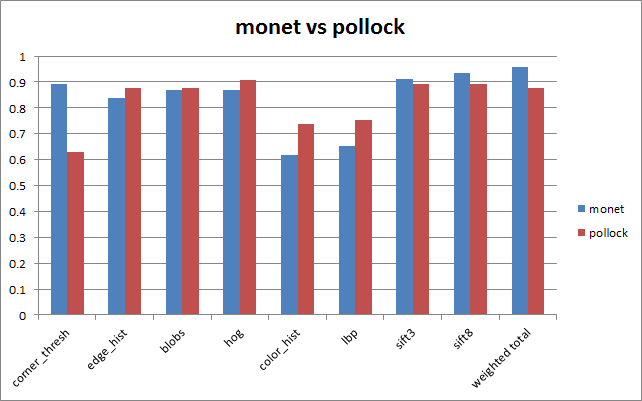
\includegraphics[width=3.5in]{graphs/monet_pollock.png}
      \caption{Monet vs Pollock}
    \end{center}
  \end{figure} \\

  Figure 3 highlights the uniqueness of Rembrandt, as his
  works are identifiable --- in some cases highly so --- by every stylometry.
  Here, the greatest distinguishing feature is not the overall weighted metric,
  but rather the color histogram. The color histogram was suspected to be a poor
  indicator of artist, but in fact it is proving to be wildly successful for
  distinguishing Monet and Rembrandt. This would suggest that either each skews
  wildly to one color, which is unlikely, or that, more likely, Rembrandt's dark
  tones are setting him apart from Monet.
  \begin{figure}[h!]
    \begin{center}
      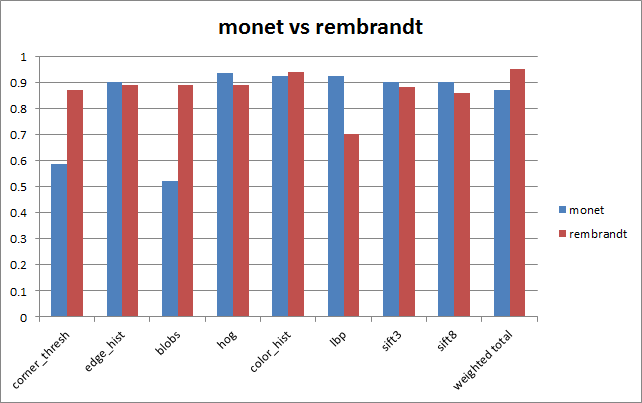
\includegraphics[width=3.5in]{graphs/monet_rembrandt.png}
      \caption{Monet vs Rembrandt}
    \end{center}
  \end{figure} \\

  We can see in Figure 4 that edge histograms were the greatest decider between
  Picasso and Pollock. It is unusual to note the the overall weighted decider
  did not pick them as well as any individual feature did (although precedent
  has certainly been set), but it is more unusual to note that the overall
  weighted decided was less by so much. LBP failed spectacularly on Picasso,
  which is unsurprising since Picasso's style has such range.
  \begin{figure}[h!]
    \begin{center}
      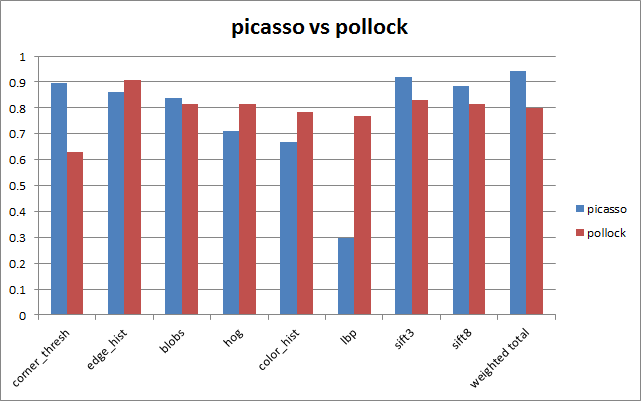
\includegraphics[width=3.5in]{graphs/picasso_pollock.png}
      \caption{Picasso vs Pollock}
    \end{center}
  \end{figure} \\

  In Figure 5, we see that SIFT 8 was the greatest decider among the features,
  and the fact that its superb success rate did not translate into the overall
  weighted decided means that a majority of the other features disagreed with
  SIFT at the same time, lending credence to the idea that there are a few
  specific paintings that did not lend themselves to our analysis. We can see
  that Rembrandt was more identifiable that Picasso from this graph.
  \begin{figure}[h!]
    \begin{center}
      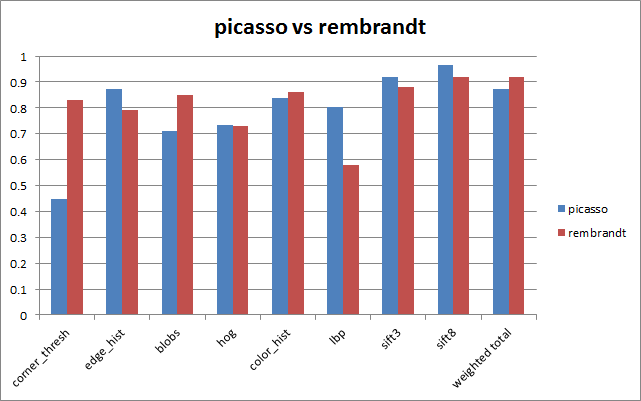
\includegraphics[width=3.5in]{graphs/picasso_rembrandt.png}
      \caption{Picasso vs Rembrandt}
    \end{center}
  \end{figure} \\

  Pollock and Rembrandt, the least identifiable and the most identifiable, in
  Figure 6 show us that we can achieve great success rates. Overall, we were
  able to identify Rembrant 100\% of the time. LBP did the worst out of any
  stylometry, measuring just under 70\% at its worst for Rembrandt and just over
  80\% for Pollock. Blob detection and edge histograms did phenomenally and
  outperformed SIFT, which has traditionally been the strongest stylometry. This
  suggests that Pollock's abstract paintings are, intuitively, more visually
  distracting than Rembrandt's dark scenes.
  \begin{figure}[h!]
    \begin{center}
      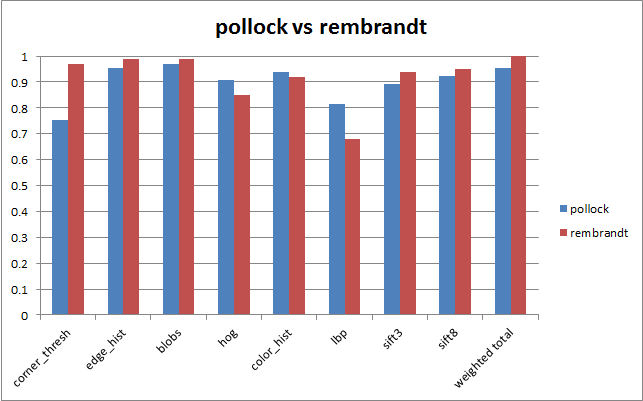
\includegraphics[width=3.5in]{graphs/pollock_rembrandt.png}
      \caption{Pollock vs Rembrandt}
    \end{center}
  \end{figure} \\

  \section{Conclusions}
  Overall, we are very pleased with the results we achieved. Our roughly 91\% overall
  identification rate is superior to that of which many individuals are capable.
  Moreover, we believe that our project lays solid groundwork for anyone looking
  to tweak or improve our algorithm. Addition of new feature detectors is
  trivial with the way our program is structured, and changing the weights of
  each feature is exceedingly simple. Our program also allows for feature data
  to be computed prior to classification and stored for later use. This allows
  for maximal preprocessing to be done on a fast machine or for an extended
  amount of time, and the data to be reused as parameters of the algorithm are
  tweaked. Below, we will discuss some generalities of the performance of our
  algorithm. We discuss the across-the-board performance of each feature
  detector, as well as the identifiability of each individual artist. \\

  Figure 7 is a very telling graph: it tells us what our most reliable measures
  are, as well as the most unreliable. We can see that, apart from the weighted
  total, the best-performing algorithms tend to be SIFT, edge histograms, and blobs.
  Corner threshhold and local binary patterns performed the worst, with HoG and
  color histograph falling somewhere in between. Importantly, we can use these
  performance measures to gain some sort of idea of how to weight their
  importance when all of the features are combined. Out of all features, though,
  the best-performing one is still the weighted total. This is highly desirable
  (and, in fact, almost necessary), since otherwise selecting just one feature
  would be ideal. The weights of each feature were initially selected based on
  the performance of the feature, and then tweaked by hand to maximize the
  performance. 
  \begin{figure}[h!]
    \begin{center}
      \includegraphics[width=3.5in]{graphs/feature_performance.png}
      \caption{Overall feature performance}
    \end{center}
  \end{figure} \\

  Figure 8 shows how often each artist was correctly identified by the
  weighted total algorithm. It can be seen that Rembrandt is the most easily
  identified artist (with 96\% accuracy) while Pollock is the least identifiable
  (88\% accuracy). Monet and Picasso fall somewhere in between (92\% and 89\%,
  respectively). It is important to note, however, that these numbers are a
  function of the weighting chosen in the weighted total algorithm. For instance,
  Pollock is frequently misidentified by the corner threshold algorithm, so a
  weight vector favoring corner threshold will yield poor results for Pollock,
  where it might yield better results for Rembrandt. 
  \begin{figure}[h!]
    \begin{center}
      \includegraphics[width=3.5in]{graphs/artist_identify.png}
      \caption{Artist identifiability}
    \end{center}
  \end{figure} \\

  \begin{thebibliography}{1}
    \bibitem{blessing} Blessing, A. and Wen, K.,
    2010,
    \emph{Using Machine Learning for Identification of Art Paintings}.
  
    \bibitem{empirical} Hughes, J. M., Mao, D., Rockmore, D. M.,
    Wang, Y., Wu, Qiang.,
    NOVEMBER 2012,
    \emph{Empirical Mode Decomposition Analysis for Visual Stylometry}.
    IEEE TRANSACTIONS ON PATTERN ANALYSIS AND MACHINE INTELLIGENCE,
    VOL. 34,
    NO. 11.
  
    \bibitem{drawing} Hughes, J. M., Graham, D. J., Rockmore, D. M.,
    \emph{Stylometrics of artwork: uses and limitations}.

    \bibitem{code} http://github.com/seydar/art\_classifier
  
  \end{thebibliography}

\end{document}

